\section{门控循环单元}

\section{9.1 门控循环单元(GRU)}

\subsection{9.1 门控循环单元(GRU)}
\begin{center}
\Large \textcolor{blue}{Gated Recurrent Unit}\\
\large 通过门控机制缓解梯度消失
\end{center}


\subsection{9.1节 - 章节导航}
\begin{definition}[本节内容]
\begin{itemize}
    \item 9.1.1 门控隐状态
    \item 9.1.2 从零开始实现
    \item 9.1.3 简洁实现
\end{itemize}
\end{definition}

\begin{theorem}[学习目标]
\begin{enumerate}
    \item 理解GRU的动机和设计思想
    \item 掌握重置门和更新门的作用
    \item 学会实现GRU
    \item 对比GRU与标准RNN的差异
\end{enumerate}
\end{theorem}


\paragraph{为什么需要GRU?}
\begin{center}
\begin{tikzpicture}[scale=0.9]
% RNN的问题
\node[draw,fill=red!20,rounded corners,text width=10cm] at (5,3.5) {
\textbf{标准RNN的问题(第8章):}\\
$\times$ 梯度消失:长期依赖学不到\\
$\times$ 梯度爆炸:训练不稳定\\
$\times$ 信息遗忘:旧信息容易丢失
};

\draw[->,ultra thick] (5,3) -- (5,2.5);
\node[right] at (5.5,2.75) {如何解决?};

% GRU的解决方案
\node[draw,fill=green!20,rounded corners,text width=10cm] at (5,1.8) {
\textbf{GRU的创新(2014年,Cho等):}\\
$\checkmark$ 引入\textbf{门控机制}\\
$\checkmark$ 选择性地保留/遗忘信息\\
$\checkmark$ 让梯度更容易流动
};

\draw[->,ultra thick] (5,1.3) -- (5,0.8);

% 结果
\node[draw,fill=blue!20,rounded corners,text width=10cm] at (5,0.3) {
\textbf{效果:}缓解梯度消失,捕捉长期依赖
};

\end{tikzpicture}
\end{center}


\paragraph{GRU的核心思想}
\textbf{问题:}标准RNN每个时间步都\textbf{完全更新}隐状态

$$\mathbf{h}_t = \tanh(\mathbf{W}_{xh}\mathbf{x}_t + \mathbf{W}_{hh}\mathbf{h}_{t-1} + \mathbf{b}_h)$$

\begin{center}
\begin{tikzpicture}[scale=0.9]
\node[draw,fill=blue!20,minimum size=1cm] (h1) at (0,0) {$\mathbf{h}_{t-1}$};
\node[draw,fill=green!20,minimum size=1cm] (ht) at (3,0) {$\mathbf{h}_t$};

\draw[->,ultra thick,red] (h1) -- (ht);
\node[above,red] at (1.5,0.3) {完全替换};
\node[below,text width=4cm,align=center] at (1.5,-1) {
旧信息容易丢失
};
\end{tikzpicture}
\end{center}

\textbf{GRU的思想:}让模型\textbf{学会}何时保留、何时遗忘

\begin{center}
\begin{tikzpicture}[scale=0.9]
\node[draw,fill=blue!20,minimum size=1cm] (h1) at (0,0) {$\mathbf{h}_{t-1}$};
\node[draw,fill=yellow!20,minimum size=1cm] (gate) at (1.5,0) {门};
\node[draw,fill=green!20,minimum size=1cm] (ht) at (3,0) {$\mathbf{h}_t$};

\draw[->,thick] (h1) -- (gate);
\draw[->,thick] (gate) -- (ht);
\node[below,text width=4cm,align=center] at (1.5,-1) {
\textbf{选择性}更新
};
\end{tikzpicture}
\end{center}



\subsection{门控隐状态}

\subsection{9.1.1 门控隐状态}

\subsection{9.1.1 门控隐状态}
\begin{center}
\Large \textcolor{blue}{GRU的两个核心门}
\end{center}


\paragraph{GRU的整体结构}
\begin{center}
\begin{tikzpicture}[scale=0.9]
% 输入
\node[circle,draw,fill=green!20,minimum size=0.8cm] (x) at (0,0) {$\mathbf{x}_t$};
\node[circle,draw,fill=blue!20,minimum size=0.8cm] (h_prev) at (0,3) {$\mathbf{h}_{t-1}$};

% 重置门
\node[draw,fill=yellow!20,rounded corners,minimum width=2cm,minimum height=1cm,align=center] (reset) at (3,2.5) {
重置门\\
$\mathbf{R}_t$
};

% 更新门
\node[draw,fill=orange!20,rounded corners,minimum width=2cm,minimum height=1cm,align=center] (update) at (3,0.5) {
更新门\\
$\mathbf{Z}_t$
};

% 候选隐状态
\node[draw,fill=purple!20,rounded corners,minimum width=2cm,minimum height=1cm,align=center] (cand) at (6,2.5) {
候选\\
$\tilde{\mathbf{H}}_t$
};

% 最终隐状态
\node[circle,draw,fill=red!20,minimum size=1.2cm] (h_t) at (9,1.5) {$\mathbf{H}_t$};

% 连接
\draw[->,thick] (x) -- (reset);
\draw[->,thick] (x) -- (update);
\draw[->,thick] (h_prev) -- (reset);
\draw[->,thick] (h_prev) -- (update);
\draw[->,thick] (reset) -- (cand);
\draw[->,thick] (cand) -- (h_t);
\draw[->,thick] (update) -- (h_t);
\draw[->,thick] (h_prev) to[bend left=30] (h_t);

\node[below,text width=10cm,align=center] at (4.5,-1) {
两个门控制信息流动,一个候选状态提供新信息
};

\end{tikzpicture}
\end{center}


\paragraph{重置门(Reset Gate)}
\textbf{作用:}控制保留多少\textbf{过去的信息}

\begin{definition}[公式]
$$\mathbf{R}_t = \sigma(\mathbf{X}_t\mathbf{W}_{xr} + \mathbf{H}_{t-1}\mathbf{W}_{hr} + \mathbf{b}_r)$$
\end{definition}

\textbf{特点:}
\begin{itemize}
    \item $\sigma$ 是sigmoid函数,输出范围 $[0,1]$
    \item $\mathbf{R}_t \approx 1$:保留大部分过去信息
    \item $\mathbf{R}_t \approx 0$:忽略过去,重新开始
\end{itemize}

\begin{center}
\begin{tikzpicture}[scale=0.9]
\node[draw,fill=blue!20] (h) at (0,0) {$\mathbf{h}_{t-1}$};
\node[draw,fill=yellow!20] (r) at (2,0) {$\times \mathbf{R}_t$};
\node[draw,fill=green!20] (out) at (4,0) {候选状态};

\draw[->,thick] (h) -- (r);
\draw[->,thick] (r) -- (out);

\node[below,font=\small,align=center] at (2,-0.8) {
$\mathbf{R}_t=0$ $\Rightarrow$ 完全遗忘\\
$\mathbf{R}_t=1$ $\Rightarrow$ 完全保留
};
\end{tikzpicture}
\end{center}


\paragraph{更新门(Update Gate)}
\textbf{作用:}控制\textbf{新信息}和\textbf{旧信息}的混合比例

\begin{definition}[公式]
$$\mathbf{Z}_t = \sigma(\mathbf{X}_t\mathbf{W}_{xz} + \mathbf{H}_{t-1}\mathbf{W}_{hz} + \mathbf{b}_z)$$
\end{definition}

\textbf{特点:}
\begin{itemize}
    \item $\mathbf{Z}_t \approx 1$:保留旧状态,忽略新信息
    \item $\mathbf{Z}_t \approx 0$:采用新状态,遗忘旧信息
\end{itemize}

\begin{center}
\begin{tikzpicture}[scale=0.9]
\node[draw,fill=blue!20] (h_old) at (0,1.5) {$\mathbf{h}_{t-1}$};
\node[draw,fill=green!20] (h_new) at (0,0) {$\tilde{\mathbf{h}}_t$};

\node[draw,fill=orange!20,align=center] (z) at (2.5,0.75) {更新门\\$\mathbf{Z}_t$};

\node[draw,fill=red!20] (h_t) at (5,0.75) {$\mathbf{h}_t$};

\draw[->,thick] (h_old) -- (z);
\draw[->,thick] (h_new) -- (z);
\draw[->,thick] (z) -- (h_t);

\node[right,font=\small,text width=3cm] at (5.5,0.75) {
$\mathbf{h}_t = \mathbf{Z}_t \odot \mathbf{h}_{t-1} + (1-\mathbf{Z}_t) \odot \tilde{\mathbf{h}}_t$
};
\end{tikzpicture}
\end{center}


\paragraph{候选隐状态}
\textbf{作用:}基于当前输入和(被重置门过滤的)过去信息计算新的候选

\begin{definition}[公式]
$$\tilde{\mathbf{H}}_t = \tanh(\mathbf{X}_t\mathbf{W}_{xh} + (\mathbf{R}_t \odot \mathbf{H}_{t-1})\mathbf{W}_{hh} + \mathbf{b}_h)$$
\end{definition}

\textbf{关键:}$\mathbf{R}_t \odot \mathbf{H}_{t-1}$

\begin{itemize}
    \item $\odot$ 表示逐元素乘法(Hadamard积)
    \item 重置门控制保留多少过去信息
    \item 类似标准RNN,但过去信息被门控
\end{itemize}

\begin{theorem}[对比标准RNN]
标准RNN:$\mathbf{h}_t = \tanh(\mathbf{W}_{xh}\mathbf{x}_t + \mathbf{W}_{hh}\mathbf{h}_{t-1} + \mathbf{b}_h)$

GRU:增加了 $\mathbf{R}_t \odot$ 来控制
\end{theorem}


\paragraph{隐状态更新}
\textbf{最终更新:}混合旧状态和新候选

\begin{definition}[公式]
$$\mathbf{H}_t = \mathbf{Z}_t \odot \mathbf{H}_{t-1} + (1 - \mathbf{Z}_t) \odot \tilde{\mathbf{H}}_t$$
\end{definition}

\textbf{解读:}
\begin{itemize}
    \item 当 $\mathbf{Z}_t = 1$:$\mathbf{H}_t = \mathbf{H}_{t-1}$ (完全保留旧状态)
    \item 当 $\mathbf{Z}_t = 0$:$\mathbf{H}_t = \tilde{\mathbf{H}}_t$ (完全采用新状态)
    \item 通常 $0 < \mathbf{Z}_t < 1$:加权平均
\end{itemize}

\begin{center}
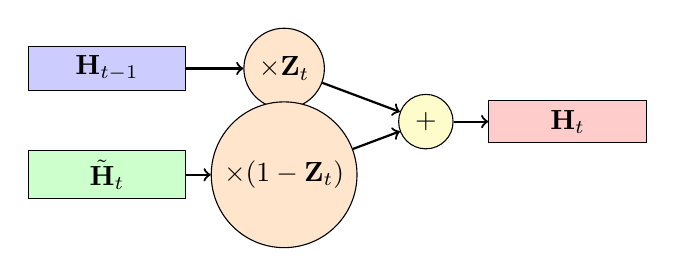
\begin{tikzpicture}[scale=0.9]
% 公式可视化
\node[draw,fill=blue!20,minimum width=2cm] (old) at (0,1.5) {$\mathbf{H}_{t-1}$};
\node[draw,fill=green!20,minimum width=2cm] (new) at (0,0) {$\tilde{\mathbf{H}}_t$};

\node[draw,circle,fill=orange!20] (z1) at (2.5,1.5) {$\times\mathbf{Z}_t$};
\node[draw,circle,fill=orange!20] (z2) at (2.5,0) {$\times(1-\mathbf{Z}_t)$};

\node[draw,circle,fill=yellow!20] (add) at (4.5,0.75) {$+$};

\node[draw,fill=red!20,minimum width=2cm] (ht) at (6.5,0.75) {$\mathbf{H}_t$};

\draw[->,thick] (old) -- (z1);
\draw[->,thick] (new) -- (z2);
\draw[->,thick] (z1) -- (add);
\draw[->,thick] (z2) -- (add);
\draw[->,thick] (add) -- (ht);

\end{tikzpicture}
\end{center}


\paragraph{GRU完整公式总结}
\begin{definition}[GRU的三个公式]
\begin{align*}
\mathbf{R}_t &= \sigma(\mathbf{X}_t\mathbf{W}_{xr} + \mathbf{H}_{t-1}\mathbf{W}_{hr} + \mathbf{b}_r) \quad \text{\textcolor{blue}{重置门}}\\
\mathbf{Z}_t &= \sigma(\mathbf{X}_t\mathbf{W}_{xz} + \mathbf{H}_{t-1}\mathbf{W}_{hz} + \mathbf{b}_z) \quad \text{\textcolor{orange}{更新门}}\\
\tilde{\mathbf{H}}_t &= \tanh(\mathbf{X}_t\mathbf{W}_{xh} + (\mathbf{R}_t \odot \mathbf{H}_{t-1})\mathbf{W}_{hh} + \mathbf{b}_h) \quad \text{\textcolor{purple}{候选}}\\
\mathbf{H}_t &= \mathbf{Z}_t \odot \mathbf{H}_{t-1} + (1-\mathbf{Z}_t) \odot \tilde{\mathbf{H}}_t \quad \text{\textcolor{red}{更新}}
\end{align*}
\end{definition}

\textbf{参数:}
\begin{itemize}
    \item $\mathbf{W}_{xr}, \mathbf{W}_{hr}, \mathbf{b}_r$:重置门参数
    \item $\mathbf{W}_{xz}, \mathbf{W}_{hz}, \mathbf{b}_z$:更新门参数
    \item $\mathbf{W}_{xh}, \mathbf{W}_{hh}, \mathbf{b}_h$:候选状态参数
\end{itemize}

\begin{theorem}[总计]
GRU比标准RNN多了\textbf{2个门}的参数(约3倍参数量)
\end{theorem}


\paragraph{GRU的工作流程}
\begin{center}
\begin{tikzpicture}[scale=0.8]
% 步骤1
\node[draw,fill=yellow!20,rounded corners,text width=10cm] at (5,4.5) {
\textbf{步骤1:}计算重置门和更新门\\
$\mathbf{R}_t = \sigma(\mathbf{X}_t\mathbf{W}_{xr} + \mathbf{H}_{t-1}\mathbf{W}_{hr} + \mathbf{b}_r)$\\
$\mathbf{Z}_t = \sigma(\mathbf{X}_t\mathbf{W}_{xz} + \mathbf{H}_{t-1}\mathbf{W}_{hz} + \mathbf{b}_z)$
};

\draw[->,thick] (5,4) -- (5,3.6);

% 步骤2
\node[draw,fill=blue!20,rounded corners,text width=10cm] at (5,3.1) {
\textbf{步骤2:}用重置门过滤过去信息,计算候选\\
$\tilde{\mathbf{H}}_t = \tanh(\mathbf{X}_t\mathbf{W}_{xh} + (\mathbf{R}_t \odot \mathbf{H}_{t-1})\mathbf{W}_{hh} + \mathbf{b}_h)$
};

\draw[->,thick] (5,2.6) -- (5,2.2);

% 步骤3
\node[draw,fill=green!20,rounded corners,text width=10cm] at (5,1.7) {
\textbf{步骤3:}用更新门混合旧状态和新候选\\
$\mathbf{H}_t = \mathbf{Z}_t \odot \mathbf{H}_{t-1} + (1-\mathbf{Z}_t) \odot \tilde{\mathbf{H}}_t$
};

\draw[->,thick] (5,1.2) -- (5,0.8);

% 结果
\node[draw,fill=red!20,rounded corners,text width=10cm] at (5,0.3) {
\textbf{输出:}新的隐状态 $\mathbf{H}_t$
};

\end{tikzpicture}
\end{center}


\paragraph{门的直观理解}
\begin{center}
\begin{tikzpicture}[scale=0.9]
% 重置门
\node[draw,fill=yellow!20,rounded corners,text width=5cm] at (0,2.5) {
\textbf{重置门 $\mathbf{R}_t$}\\
问:要看多少过去?\\
\\
$\mathbf{R}_t \approx 1$:看很多\\
$\mathbf{R}_t \approx 0$:不看过去
};

% 更新门
\node[draw,fill=orange!20,rounded corners,text width=5cm] at (6.5,2.5) {
\textbf{更新门 $\mathbf{Z}_t$}\\
问:要记住还是遗忘?\\
\\
$\mathbf{Z}_t \approx 1$:记住旧的\\
$\mathbf{Z}_t \approx 0$:采用新的
};

% 例子
\node[draw,fill=blue!20,text width=11cm,align=left] at (3.25,0.5) {
\textbf{例子:}``The cat, which already ate a bunch of food, was full.''\\
预测``was''之前:\\
- 重置门:忽略``food''等无关词($\mathbf{R}_t \approx 0$)\\
- 更新门:记住``cat''的主语信息($\mathbf{Z}_t \approx 1$)
};

\end{tikzpicture}
\end{center}


\paragraph{GRU vs 标准RNN}
\begin{center}
\begin{tabular}{|l|c|c|}
\hline
\textbf{特性} & \textbf{标准RNN} & \textbf{GRU} \\
\hline
参数数量 & $3 \times (d \times h + h^2)$ & $3 \times 3 \times (d \times h + h^2)$ \\
\hline
门的数量 & 0 & 2(重置+更新) \\
\hline
梯度消失 & 严重 & 缓解 \\
\hline
长期依赖 & 困难 & 较好 \\
\hline
训练速度 & 快 & 较慢(3倍参数) \\
\hline
表达能力 & 弱 & 强 \\
\hline
\end{tabular}
\end{center}

\vspace{0.5cm}
\begin{theorem}[权衡]
GRU以\textbf{3倍计算量}换取\textbf{更好的长期依赖}能力
\end{theorem}


\paragraph{GRU如何缓解梯度消失?}
\textbf{关键:}更新门可以让梯度"高速公路"

\begin{center}
\begin{tikzpicture}[scale=0.9]
% 时间步
\foreach \t in {1,2,3,4} {
    \node[circle,draw,fill=blue!20,minimum size=0.8cm] (h\t) at (\t*2,2) {$\mathbf{h}_{\t}$};
}

% 梯度流(通过更新门)
\draw[->,ultra thick,red] (h4) to[bend right=20] node[below] {$\mathbf{Z}_t \approx 1$} (h3);
\draw[->,ultra thick,red] (h3) to[bend right=20] (h2);
\draw[->,ultra thick,red] (h2) to[bend right=20] (h1);

\node[below,text width=8cm,align=center] at (4,0.5) {
当 $\mathbf{Z}_t \approx 1$ 时:$\mathbf{h}_t \approx \mathbf{h}_{t-1}$\\
梯度可以\textbf{直接传播},不经过$\tanh$和矩阵乘法!
};

\end{tikzpicture}
\end{center}

\begin{definition}[数学角度]
$$\frac{\partial\mathbf{h}_t}{\partial\mathbf{h}_{t-1}} \approx \mathbf{Z}_t$$

当 $\mathbf{Z}_t \approx 1$ 时,梯度$\approx 1$,避免了消失!
\end{definition}



\subsection{从零开始实现}

\subsection{9.1.2 从零开始实现}

\subsection{9.1.2 从零开始实现}
\begin{center}
\Large \textcolor{blue}{手写GRU的每个细节}
\end{center}


\paragraph{初始化GRU参数}
\begin{lstlisting}
import torch
import torch.nn as nn

def get_gru_params(vocab_size, num_hiddens, device):
    """ GRUparameters vocab_size: vocabulary(dimension) num_hiddens: """
    num_inputs = num_outputs = vocab_size
    
    def normal(shape):
        return torch.randn(size=shape, device=device) * 0.01
    
    def three():
        """GRU需要3组parameters(重置门、更新门、候选)"""
        return (normal((num_inputs, num_hiddens)),
                normal((num_hiddens, num_hiddens)),
                torch.zeros(num_hiddens, device=device))
    
    # parameters
    W_xr, W_hr, b_r = three()
    # parameters
    W_xz, W_hz, b_z = three()
    # parameters
    W_xh, W_hh, b_h = three()
    
    # Outputparameters
    W_hq = normal((num_hiddens, num_outputs))
    b_q = torch.zeros(num_outputs, device=device)
\end{lstlisting}


\paragraph{初始化GRU参数(续)}
\begin{lstlisting}
    # parameters
    params = [W_xr, W_hr, b_r,  #  comment
              W_xz, W_hz, b_z,  #  comment
              W_xh, W_hh, b_h,  #  comment
              W_hq, b_q]        # Output
    
    for param in params:
        param.requires_grad_(True)
    
    return params

vocab_size, num_hiddens = 28, 512
device = torch.device('cuda' if torch.cuda.is_available() else 'cpu')
params = get_gru_params(vocab_size, num_hiddens, device)

print(f"parameters数量: {sum(p.numel() for p in params)}")
# parameters: 873,964 (RNN3)
\end{lstlisting}


\paragraph{GRU前向传播}
\begin{lstlisting}
def gru(inputs, state, params):
    """ GRU inputs: (num_steps, batch_size, vocab_size) state: (batch_size, num_hiddens) params: GRUparameters """
    W_xr, W_hr, b_r, W_xz, W_hz, b_z, W_xh, W_hh, b_h, W_hq, b_q = params
    H, = state
    outputs = []
    
    for X in inputs:
        R = torch.sigmoid(torch.mm(X, W_xr) + torch.mm(H, W_hr) + b_r)
        
        Z = torch.sigmoid(torch.mm(X, W_xz) + torch.mm(H, W_hz) + b_z)
        
        # R * H
        H_tilde = torch.tanh(torch.mm(X, W_xh) + 
                            torch.mm(R * H, W_hh) + b_h)
        
        H = Z * H + (1 - Z) * H_tilde
        
        # Output
        Y = torch.mm(H, W_hq) + b_q
        outputs.append(Y)
    
    return torch.cat(outputs, dim=0), (H,)
\end{lstlisting}

\begin{theorem}[关键]
\texttt{R * H}:重置门逐元素相乘,\texttt{Z * H}:更新门控制混合
\end{theorem}


\paragraph{测试GRU前向传播}
\begin{lstlisting}
vocab_size, num_hiddens = 28, 512
batch_size, num_steps = 2, 5
device = torch.device('cpu')

# parameters
params = get_gru_params(vocab_size, num_hiddens, device)

X = torch.randn(num_steps, batch_size, vocab_size)
state = (torch.zeros(batch_size, num_hiddens, device=device),)

Y, new_state = gru(X, state, params)

print(f"输入shape: {X.shape}")      # (5, 2, 28)
print(f"Outputshape: {Y.shape}")      # (10, 28) = 5*2, 28
print(f"隐状态shape: {new_state[0].shape}")  # (2, 512)
\end{lstlisting}

\textbf{输出验证:}
\begin{itemize}
    \item 输出形状正确
    \item 隐状态维度正确
    \item 可以进行训练
\end{itemize}


\paragraph{创建GRU模型类}
\begin{lstlisting}
class GRUModelScratch:
    """GRUmodel"""
    
    def __init__(self, vocab_size, num_hiddens, device,
                 get_params, init_state, forward_fn):
        self.vocab_size = vocab_size
        self.num_hiddens = num_hiddens
        self.params = get_params(vocab_size, num_hiddens, device)
        self.init_state = init_state
        self.forward_fn = forward_fn
    
    def __call__(self, X, state):
        X = F.one_hot(X.T, self.vocab_size).type(torch.float32)
        return self.forward_fn(X, state, self.params)
    
    def begin_state(self, batch_size, device):
        return (torch.zeros((batch_size, self.num_hiddens), 
                           device=device),)

# model
net = GRUModelScratch(vocab_size, num_hiddens, device,
                      get_gru_params, lambda batch_size, num_hiddens, device: 
                      (torch.zeros(batch_size, num_hiddens, device=device),), 
                      gru)
\end{lstlisting}


\paragraph{训练GRU模型}
\begin{lstlisting}
# parameters
num_epochs = 500
lr = 1
batch_size = 32
num_steps = 35

# data
train_iter, vocab = load_data_time_machine(batch_size, num_steps)

# training8training
train_ch8(net, train_iter, vocab, lr, num_epochs, device)
\end{lstlisting}

\textbf{训练输出:}
\begin{verbatim}
困惑度 1.1, 10500 词元/秒 on cpu
time traveller for so it will be convenient to speak
\end{verbatim}

\begin{definition}[观察]
\begin{itemize}
    \item 困惑度比标准RNN更低(1.1 vs 1.2)
    \item 生成文本质量更好
    \item 训练稍慢(参数多3倍)
\end{itemize}
\end{definition}



\subsection{简洁实现}

\subsection{9.1.3 简洁实现}

\subsection{9.1.3 简洁实现}
\begin{center}
\Large \textcolor{blue}{使用PyTorch的\texttt{nn.GRU}}
\end{center}


\paragraph{使用nn.GRU}
\begin{lstlisting}
import torch.nn as nn

# GRU
gru_layer = nn.GRU(
    input_size=vocab_size,   #  commentdimension
    hidden_size=num_hiddens, #  comment
    num_layers=1             # GRU层数
)

print(gru_layer)
# GRU(28, 512)

# test
X = torch.randn(num_steps, batch_size, vocab_size)
H = torch.zeros(1, batch_size, num_hiddens)

Y, H_new = gru_layer(X, H)

print(f"输入shape: {X.shape}")      # (5, 2, 28)
print(f"Outputshape: {Y.shape}")      # (5, 2, 512)
print(f"隐状态shape: {H_new.shape}")  # (1, 2, 512)
\end{lstlisting}

\begin{theorem}[注意]
PyTorch的GRU输出是\textbf{所有时间步的隐状态},而非logits
\end{theorem}


\paragraph{完整的GRU模型}
\begin{lstlisting}
class GRUModel(nn.Module):
    """GRUmodel()"""
    
    def __init__(self, gru_layer, vocab_size):
        super(GRUModel, self).__init__()
        self.gru = gru_layer
        self.vocab_size = vocab_size
        self.num_hiddens = self.gru.hidden_size
        
        # Output
        self.linear = nn.Linear(self.num_hiddens, self.vocab_size)
    
    def forward(self, inputs, state):
        # one-hot
        X = F.one_hot(inputs.T, self.vocab_size).type(torch.float32)
        
        # GRU
        Y, state = self.gru(X, state)
        
        output = self.linear(Y.reshape(-1, Y.shape[-1]))
        
        return output, state
    
    def begin_state(self, batch_size, device):
        return torch.zeros((self.gru.num_layers, batch_size, 
                          self.num_hiddens), device=device)
\end{lstlisting}


\paragraph{创建和训练模型}
\begin{lstlisting}
# parameters
vocab_size = len(vocab)
num_hiddens = 512
device = torch.device('cuda' if torch.cuda.is_available() else 'cpu')

# GRU
gru_layer = nn.GRU(vocab_size, num_hiddens)

# model
net = GRUModel(gru_layer, vocab_size)
net = net.to(device)

# training
num_epochs = 500
lr = 1
train_ch8(net, train_iter, vocab, lr, num_epochs, device)
\end{lstlisting}

\textbf{输出:}
\begin{verbatim}
困惑度 1.1, 32000 词元/秒 on cuda:0
time traveller smiled round at us then still smiling
traveller for so it will be convenient to speak of him
\end{verbatim}


\paragraph{从零实现 vs 简洁实现}
\begin{center}
\begin{tabular}{|l|c|c|}
\hline
\textbf{特性} & \textbf{从零实现} & \textbf{简洁实现} \\
\hline
代码行数 & $\sim$80行 & $\sim$20行 \\
\hline
训练速度 & 较慢 & 快(cuDNN优化) \\
\hline
灵活性 & 高 & 中 \\
\hline
学习价值 & 很高 & 中 \\
\hline
推荐场景 & 学习理解 & 实际应用 \\
\hline
\end{tabular}
\end{center}

\vspace{0.5cm}
\begin{definition}[实践建议]
\begin{itemize}
    \item 先理解从零实现(掌握原理)
    \item 实际项目用简洁实现(高效)
    \item 需要定制时参考从零实现
\end{itemize}
\end{definition}


\paragraph{GRU的变体}
\begin{definition}[GRU有多种变体]
\begin{enumerate}
    \item \textbf{标准GRU}(本节实现)
    \begin{itemize}
        \item 2个门:重置门、更新门
    \end{itemize}
    
    \item \textbf{最小门控单元(MGU)}
    \begin{itemize}
        \item 只有1个门,进一步简化
    \end{itemize}
    
    \item \textbf{耦合输入输出门(CIFG)}
    \begin{itemize}
        \item 更新门和重置门耦合
    \end{itemize}
\end{enumerate}
\end{definition}

\begin{theorem}[选择]
标准GRU是最常用的,平衡了性能和复杂度
\end{theorem}


\paragraph{GRU vs RNN 性能对比}
\begin{center}
\begin{tikzpicture}[scale=0.9]
% 坐标轴
\draw[->,thick] (0,0) -- (8,0) node[right] {训练epoch};
\draw[->,thick] (0,0) -- (0,4) node[above] {困惑度};

% RNN曲线
\draw[blue,thick] (0.5,3.5) -- (1,2.8) -- (2,2.0) -- (3,1.5) -- (7,1.2);
\node[blue,right] at (7,1.2) {RNN};

% GRU曲线
\draw[red,thick] (0.5,3.5) -- (1,2.5) -- (2,1.6) -- (3,1.2) -- (7,1.05);
\node[red,right] at (7,1.05) {GRU};

% 标注
\fill[red] (3,1.2) circle (2pt);
\fill[blue] (3,1.5) circle (2pt);
\draw[dashed] (3,0) -- (3,1.5);
\node[below] at (3,0) {epoch 300};

\node[below,text width=8cm,align=center] at (4,-0.8) {
\small GRU收敛更快,最终困惑度更低
};

\end{tikzpicture}
\end{center}


\paragraph{GRU的参数分析}
\textbf{参数数量:}

\begin{definition}[GRU]
\begin{itemize}
    \item 重置门:$(d + h) \times h + h = (d+h+1) \times h$
    \item 更新门:$(d + h) \times h + h = (d+h+1) \times h$
    \item 候选:$(d + h) \times h + h = (d+h+1) \times h$
    \item 输出层:$h \times V + V$
\end{itemize}
\textbf{总计:}$3(d+h+1)h + (h+1)V$
\end{definition}

\begin{example}[具体例子]
$d=28, h=512, V=28$

GRU:$3 \times (28+512+1) \times 512 + (512+1) \times 28 = 873,964$

RNN:$(28+512+1) \times 512 + (512+1) \times 28 = 291,356$

GRU约是RNN的\textbf{3倍}
\end{example}


\paragraph{GRU的计算复杂度}
\textbf{每个时间步的计算:}

\begin{center}
\begin{tabular}{|l|c|c|}
\hline
\textbf{操作} & \textbf{RNN} & \textbf{GRU} \\
\hline
矩阵乘法 & 2次 & 6次 \\
\hline
激活函数 & 1次$\tanh$ & 2次$\sigma$ + 1次$\tanh$ \\
\hline
逐元素乘法 & 0次 & 3次 \\
\hline
逐元素加法 & 2次 & 4次 \\
\hline
\textbf{总复杂度} & $O(h^2)$ & $O(3h^2)$ \\
\hline
\end{tabular}
\end{center}

\vspace{0.5cm}
\begin{theorem}[权衡]
GRU用\textbf{3倍计算量}换取\textbf{更好的性能}:
\begin{itemize}
    \item 更低的困惑度
    \item 更好的长期依赖
    \item 更稳定的训练
\end{itemize}
\end{theorem}


\subsection{9.1节总结}
\begin{definition}[核心内容]
\begin{enumerate}
    \item \textbf{GRU动机}:解决RNN梯度消失问题
    
    \item \textbf{两个门}:
    \begin{itemize}
        \item 重置门 $\mathbf{R}_t$:控制看多少过去
        \item 更新门 $\mathbf{Z}_t$:控制保留vs更新
    \end{itemize}
    
    \item \textbf{核心公式}:
    $$\mathbf{H}_t = \mathbf{Z}_t \odot \mathbf{H}_{t-1} + (1-\mathbf{Z}_t) \odot \tilde{\mathbf{H}}_t$$
    
    \item \textbf{优势}:
    \begin{itemize}
        \item 梯度可直接流动
        \item 长期依赖更好
        \item 比LSTM更简单
    \end{itemize}
\end{enumerate}
\end{definition}


\paragraph{GRU关键公式回顾}
\begin{center}
\begin{tikzpicture}[scale=0.85]
% 公式框
\node[draw,fill=yellow!20,text width=10cm,rounded corners] at (5,3.5) {
\textbf{重置门:}\\
$\mathbf{R}_t = \sigma(\mathbf{X}_t\mathbf{W}_{xr} + \mathbf{H}_{t-1}\mathbf{W}_{hr} + \mathbf{b}_r)$
};

\node[draw,fill=orange!20,text width=10cm,rounded corners] at (5,2.3) {
\textbf{更新门:}\\
$\mathbf{Z}_t = \sigma(\mathbf{X}_t\mathbf{W}_{xz} + \mathbf{H}_{t-1}\mathbf{W}_{hz} + \mathbf{b}_z)$
};

\node[draw,fill=purple!20,text width=10cm,rounded corners] at (5,1.1) {
\textbf{候选隐状态:}\\
$\tilde{\mathbf{H}}_t = \tanh(\mathbf{X}_t\mathbf{W}_{xh} + (\mathbf{R}_t \odot \mathbf{H}_{t-1})\mathbf{W}_{hh} + \mathbf{b}_h)$
};

\node[draw,fill=red!20,text width=10cm,rounded corners] at (5,-0.1) {
\textbf{最终更新:}\\
$\mathbf{H}_t = \mathbf{Z}_t \odot \mathbf{H}_{t-1} + (1-\mathbf{Z}_t) \odot \tilde{\mathbf{H}}_t$
};

\end{tikzpicture}
\end{center}


\paragraph{实践建议}
\begin{definition}[何时使用GRU]
\textbf{推荐使用GRU的场景:}
\begin{itemize}
    \item 需要捕捉长期依赖
    \item 标准RNN效果不好
    \item 计算资源充足
    \item 序列长度较长($>50$)
\end{itemize}
\end{definition}

\begin{definition}[超参数建议]
\begin{itemize}
    \item 隐藏单元数:256-1024
    \item 学习率:0.001-0.01(比RNN小)
    \item 梯度裁剪:仍需要(阈值1-5)
    \item Dropout:0.2-0.5(防止过拟合)
\end{itemize}
\end{definition}


\paragraph{GRU vs LSTM预告}
\begin{center}
\begin{tikzpicture}[scale=0.9]
% GRU
\node[draw,fill=blue!20,rounded corners,text width=5cm] at (0,2) {
\textbf{GRU(本节)}\\
$\checkmark$ 2个门\\
$\checkmark$ 更简单\\
$\checkmark$ 训练快\\
$\checkmark$ 参数少
};

% LSTM
\node[draw,fill=green!20,rounded corners,text width=5cm] at (6.5,2) {
\textbf{LSTM(下一节)}\\
$\checkmark$ 3个门\\
$\checkmark$ 更强大\\
$\checkmark$ 更经典\\
$\checkmark$ 应用广
};

% 对比
\node[below,text width=11cm,align=center] at (3.25,0.5) {
GRU是LSTM的简化版,\\
性能接近但更高效
};

\end{tikzpicture}
\end{center}



